\begin{abstract}
Η συγκεκριμένη διπλωματική ε\-ργα\-σία έχει στόχο την επίτευξη 
υπολογισμού της θέσης - στον τρισδιάστατο χώρο - ενός πρότυπου α\-ντι\-κειμένου, 
από ένα σμήνος drone\udot με όσο δυνατόν χαμηλότερο κόστος υλικού ανά node του 
συστήματος. Ιδανικά θα γίνει προσπάθεια να γίνει multi sensor data fusion 
και να αξιοποιηθούν πληροφορίες τόσο με βάση image-based τεχνικών υπολογισμού, 
όπως επίσης και RF-based.
\end{abstract}
  
\begin{keywords}
Drone, UAV, Swarm, OpenCV, Robot Operating System, Camera, Ultra Wide Band
\end{keywords}
%%%%%%%%%%%%%%%%%%%%%%%%%%%%%%%%%%%%%%%%%%%%%%%%%%%%%%%%%%%%%%%%%%%%%%%%%%%%%%%%

\section{INTRODUCTION}
Τα τελευταία χρόνια ο χώρος των αεροχημάτων παρουσιάζει αρκετά μεγάλο ερευνητικό 
ενδιαφέρον, με αποτέλεσμα την εμφάνιση σμηνών από drone σε ένα μεγάλο
πλήθος εφαρμογών. 

Σε αυτού του τύπου τις εφαρμογές είναι πολύ σημαντική η γνώση της θέσης του κάθε 
μεμονωμένου Unmanned Aerial Vehicle (UAV) είτε σχετικά με τα γειτονικά nodes του 
συστήματος, είτε σε συ\-νδυα\-σμό αυτού και κατά απόλυτο τρόπο\udot σύμφωνα με ένα 
καθορισμένο σύστημα αξόνων.

Παρόλη την εξέλιξη της ακρίβειας από $\small \sim$5m [\cite{1}] 
σε $\small \sim$30cm [\cite{2}] - για μη στρατιωτική χρήση - των 
Global Navigation Satellite System (GNSS)\udot
όπου όμως ούτε αυτή δεν είναι αρκετή για τις ανάγκες ορισμένων εφαρμογών, 
πολλές φορές οδηγούμαστε ή να κινηθούμε σε αρκετά ακριβές 
λύσεις όπως RTK GPS [\cite{3}], το οποίο μπορεί να προσφέρει ακρίβεια 1-2cm σε 
ακτίνες $\small \sim$20km ή να αναζητήσουμε άλλους τρόπους υπολογισμού της θέσης
των drone σε ένα swarm.

Στην υφιστάμενη βιβλιογραφία, μπορεί κανείς εύκολα να βρει μεθόδους ανεύρεση της θέσης  
των drones με τεχνικές RF, όπως μέτρηση απόστασης με 
χρήση Ultra wide band[\cite{4}], είτε με βοήθεια των πρόσφατα εισαχθέντων στην καθημερινότητα
5G δικτύων [\cite{5}] είτε με την βοήθεια καμερών [\cite{6}]. Ενώ επίσης, πολλές φορές είναι
εξίσου σημαντικό εκτός από τον υπολογισμός της θέσης των ίδιων των drone να βρούμε και την
θέση επιπλέον αντικειμένων τα οποία σχετίζονται με την εκάστοτε εφαρμογή.

\section{THESIS STATEMENT}
Όταν αναφερόμαστε σε motion capturing systems [\cite{7}], όπως το Vicon [\cite{8}] 
ή το Optitrack [\cite{9}], μιλάμε κυρίως για στατικά, εσωτερικών χώρων συστήματα 
τα οποία είναι υπεύθυνα να ανιχνεύουν και να συλλαμβάνουν την κίνηση σωμάτων.

Στην συγκεκριμένη διπλωματική εργασία θα γίνει μία πρώτη προ\-σπά\-θεια επίλυσης του 
προβλήματος υπολογισμού της θέσης ενός μεμονωμένου - γνωστών διαστάσεων - αντικειμένου 
με χρήση drones, όπως παρουσιάζεται στο Figure \ref{fig:1} με σκοπό μελλοντικά να είναι 
δυνατό το tracking αντικειμένων σε εξωτερικούς χώρους και δυναμικά περιβάλλοντα.

\begin{figure}[thpb]
  \centering
  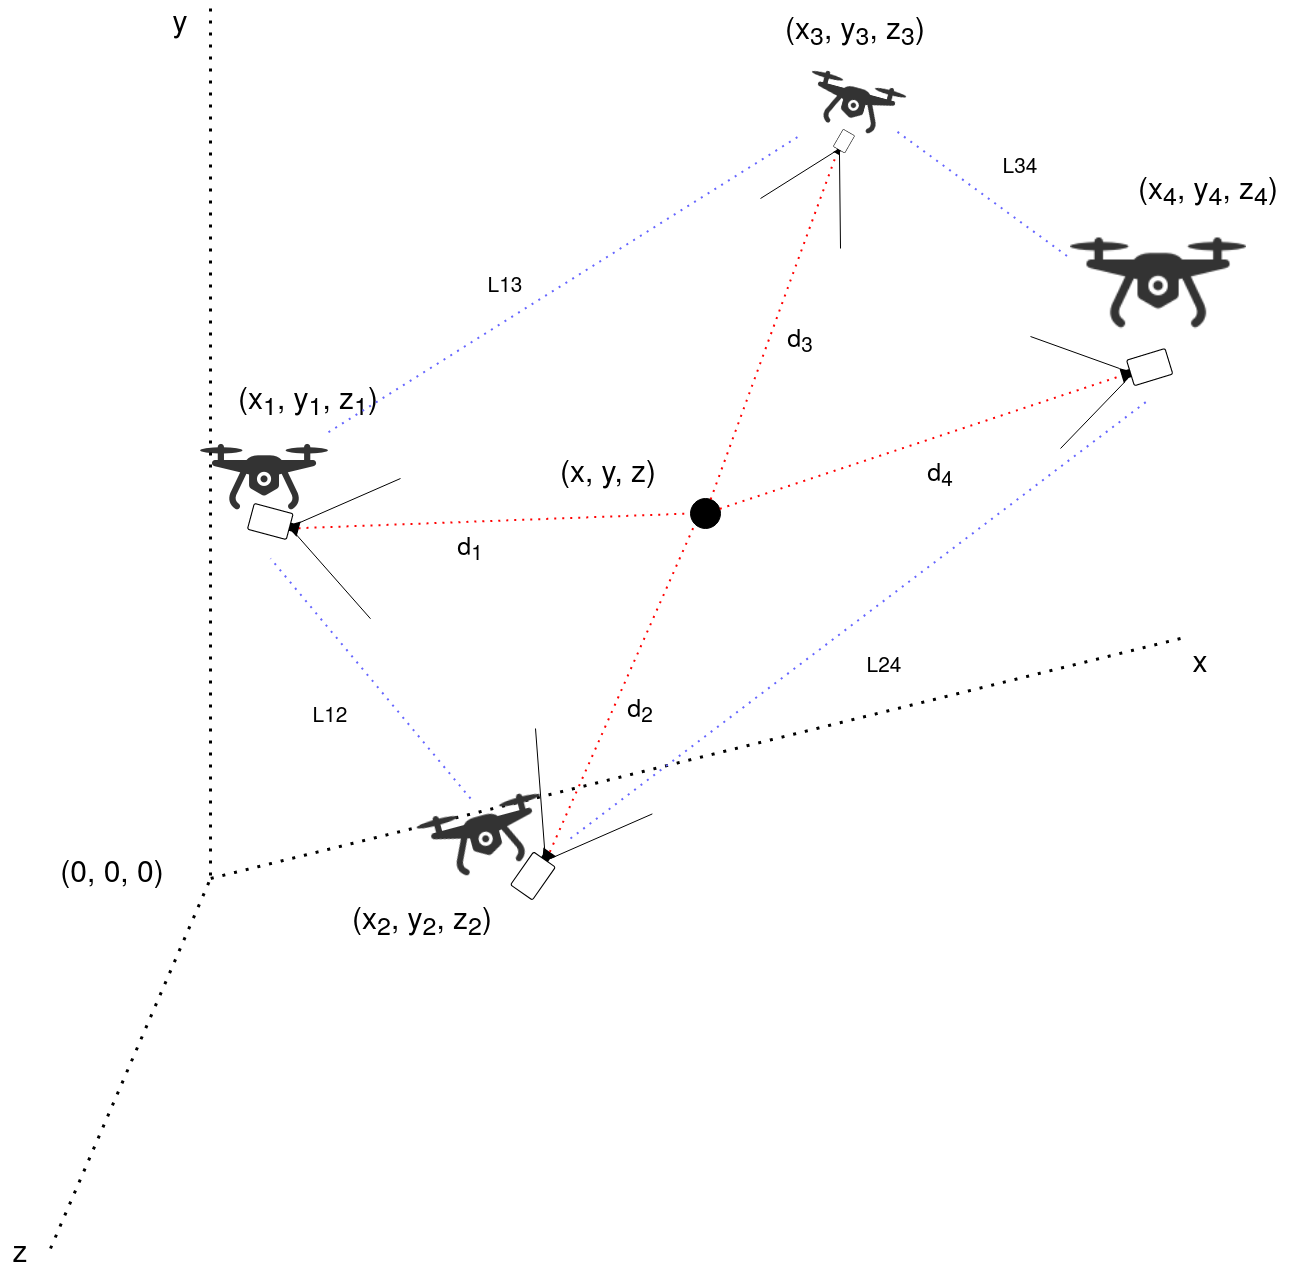
\includegraphics[width=\linewidth]{Images/3dDrones-camera-pose.png}
  \caption{Drones' cameras track object in 3D space}
  \label{fig:1}
\end{figure}

\section{APPROACH}
Ο τρόπος με τον οποίο θα γίνει προσπάθεια να λυθεί το συγκεκριμένο πρόβλημα, είναι αρχικά με χρήση 
κάμερας να εντοπιστεί το αντικείμενο στο χώρο, να απομονωθεί μόνο χρήσιμη πληροφορία για αυτό   
- όπως φαίνεται στο Figure \ref{fig:2} - και στην συνέχεια με βάση την γνώση των ακριβών του διαστάσεων
καθώς επίσης και το πλήθος των pixel που καταλαμβάνει στην κάμερα να υπολογιστεί η απόσταση που έχει από 
αυτήν. Στην συνέχεια για κάθε drone να ληφθούν πληροφορίες τις θέσεις του - μέσω GPS, IMU, κλπ αισθητήρων -
και αφού έχει γίνει το κατάλληλο φιλτράρισμα των πληροφοριών, να ομαδοποιηθούν όλες οι πληροφορίες και 
να αποσταλούν στα γειτονικά drones του συστήματος. Αφού πλέον το κάθε drone λάβει από τα γειτονικά τις 
θέσεις των υπόλοιπων καθώς και την απόσταση του αντικειμένου από αυτά, μπορεί να γίνει χρήση κατάλληλου



\begin{figure}[thpb]
  \centering
  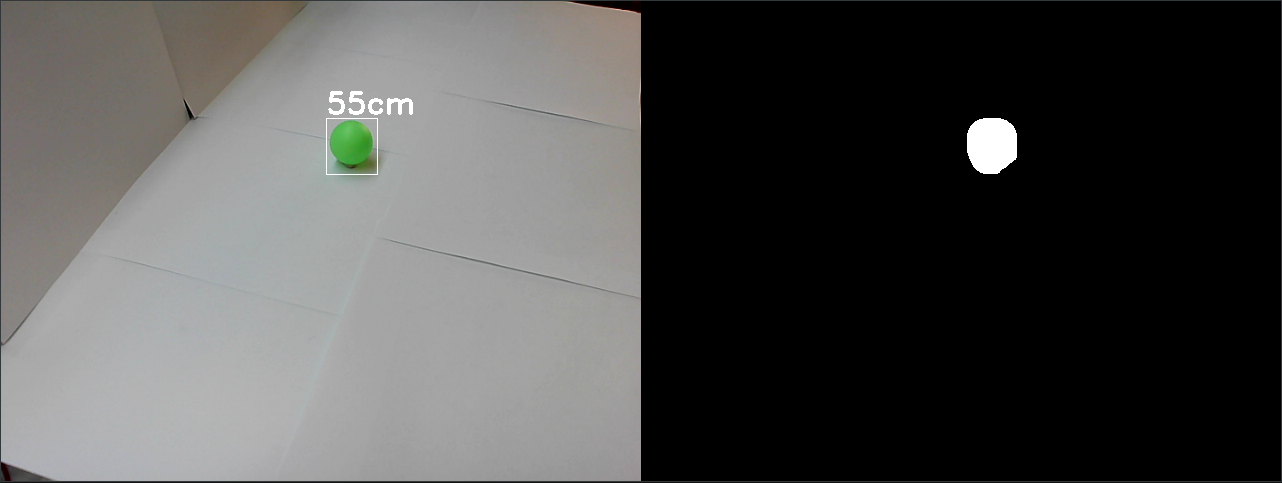
\includegraphics[width=\linewidth]{Images/Thesis-Proposal-shape-color-detection.png}
  \caption{Blob detection - σύμφωνα με το σχήμα/χρώμα - της μπάλας και υπολογισμός της απόστασης της από την κάμερα}
  \label{fig:2}
\end{figure}

\section{WORK PLAN}
Σε πρώτο επίπεδο θα αποκτηθούν γνώσεις σχετικά με την βιβλιοθήκη OpenCV, μέσω της οποίας
με οπτικό τρόπο θα εντοπιστεί το αντικείμενο για τον υπολογισμό της απόστασης του απο την
κάμερα.

Αφού 

Τέλος, σε περίπτωση όπου επιτραπεί χρονικά θα γίνει προσπάθεια διόρθωσης των σφαλμάτων του 
GPS με RF-based μεθόδων. Πιο συγκεκριμένα με μέτρηση απόστασης μεταξύ των nodes των 
νακρίβεια 5-10cm σε εμβέλεια 200m και αυτές οι αποστάσεις να συμβάλουν επίσης στον localization
algorithm.




\begin{table}[H]
  \caption[]{Raspberry Pi 4 Model B Specifications}
  \label{tab:1}
  \centering
  \begin{tabular}{ll}
      \hline
      \textbf{Feature} & \textbf{Value}  \\
      \hline
          Processor & \Centerstack{Broadcom BCM2711, Quad core Cortex-A72 \\(ARM v8) 64-bit SoC @ 1.5GHz }\\
          Memory & 8GB LPDDR4-3200 SDRAM \\
          Storage & External Micro-SD \\  
          Power & 5V DC (maximum 3A), 5-15Watt \\
          Cost & $\sim$100 €\\
          Weight & 46 grams (without case), 99 grams (with case) \\
          Peripherals & GPIO, I2C, SPI, UART \\
          \hline
  \end{tabular}
\end{table}


\begin{table}[H]
  \caption[]{Jetson Nano Developer Kit Specifications}
  \label{tab:2}
  \centering
  \begin{tabular}{ll}
      \hline
      \textbf{Feature} & \textbf{Value}  \\
      \hline
          CPU & Quad-core ARM Cortex-A57 MPCore processor\\
          GPU & \Centerstack{NVIDIA Maxwell architecture with 128 NVIDIA\\ CUDA® cores} \\
          Memory & 4 GB 64-bit LPDDR4; 25.6 gigabytes/second \\
          Storage & External Micro-SD \\  
          Power & 5V DC, 5-10Watt \\
          Cost & $\sim$120€\\
          Weight & 250 grams (without case)\\
          Peripherals & GPIO, I2C, I2S, SPI, UART \\
          \hline
  \end{tabular}
\end{table}